% Options for packages loaded elsewhere
\PassOptionsToPackage{unicode}{hyperref}
\PassOptionsToPackage{hyphens}{url}
%
\documentclass[
]{article}
\usepackage{amsmath,amssymb}
\usepackage{lmodern}
\usepackage{iftex}
\ifPDFTeX
  \usepackage[T1]{fontenc}
  \usepackage[utf8]{inputenc}
  \usepackage{textcomp} % provide euro and other symbols
\else % if luatex or xetex
  \usepackage{unicode-math}
  \defaultfontfeatures{Scale=MatchLowercase}
  \defaultfontfeatures[\rmfamily]{Ligatures=TeX,Scale=1}
\fi
% Use upquote if available, for straight quotes in verbatim environments
\IfFileExists{upquote.sty}{\usepackage{upquote}}{}
\IfFileExists{microtype.sty}{% use microtype if available
  \usepackage[]{microtype}
  \UseMicrotypeSet[protrusion]{basicmath} % disable protrusion for tt fonts
}{}
\makeatletter
\@ifundefined{KOMAClassName}{% if non-KOMA class
  \IfFileExists{parskip.sty}{%
    \usepackage{parskip}
  }{% else
    \setlength{\parindent}{0pt}
    \setlength{\parskip}{6pt plus 2pt minus 1pt}}
}{% if KOMA class
  \KOMAoptions{parskip=half}}
\makeatother
\usepackage{xcolor}
\usepackage[margin=1in]{geometry}
\usepackage{graphicx}
\makeatletter
\def\maxwidth{\ifdim\Gin@nat@width>\linewidth\linewidth\else\Gin@nat@width\fi}
\def\maxheight{\ifdim\Gin@nat@height>\textheight\textheight\else\Gin@nat@height\fi}
\makeatother
% Scale images if necessary, so that they will not overflow the page
% margins by default, and it is still possible to overwrite the defaults
% using explicit options in \includegraphics[width, height, ...]{}
\setkeys{Gin}{width=\maxwidth,height=\maxheight,keepaspectratio}
% Set default figure placement to htbp
\makeatletter
\def\fps@figure{htbp}
\makeatother
\setlength{\emergencystretch}{3em} % prevent overfull lines
\providecommand{\tightlist}{%
  \setlength{\itemsep}{0pt}\setlength{\parskip}{0pt}}
\setcounter{secnumdepth}{5}
\usepackage{graphicx}
\usepackage{hyperref}
\ifLuaTeX
  \usepackage{selnolig}  % disable illegal ligatures
\fi
\IfFileExists{bookmark.sty}{\usepackage{bookmark}}{\usepackage{hyperref}}
\IfFileExists{xurl.sty}{\usepackage{xurl}}{} % add URL line breaks if available
\urlstyle{same} % disable monospaced font for URLs
\hypersetup{
  hidelinks,
  pdfcreator={LaTeX via pandoc}}

\author{}
\date{\vspace{-2.5em}}

\begin{document}

%! Author = Niek Scholten
%! Date = 24-10-2022

%Turn off page numbering
\pagenumbering{gobble}
\begin{center}

    \Huge{Predicting bird species from their songs using machine learning}\\
    \vspace{\baselineskip}
    \LARGE{Theme 09 - Introduction Machine Learning}\\
    \large{Research paper}\\
    \vspace{\baselineskip}

    \begin{figure}
        \centering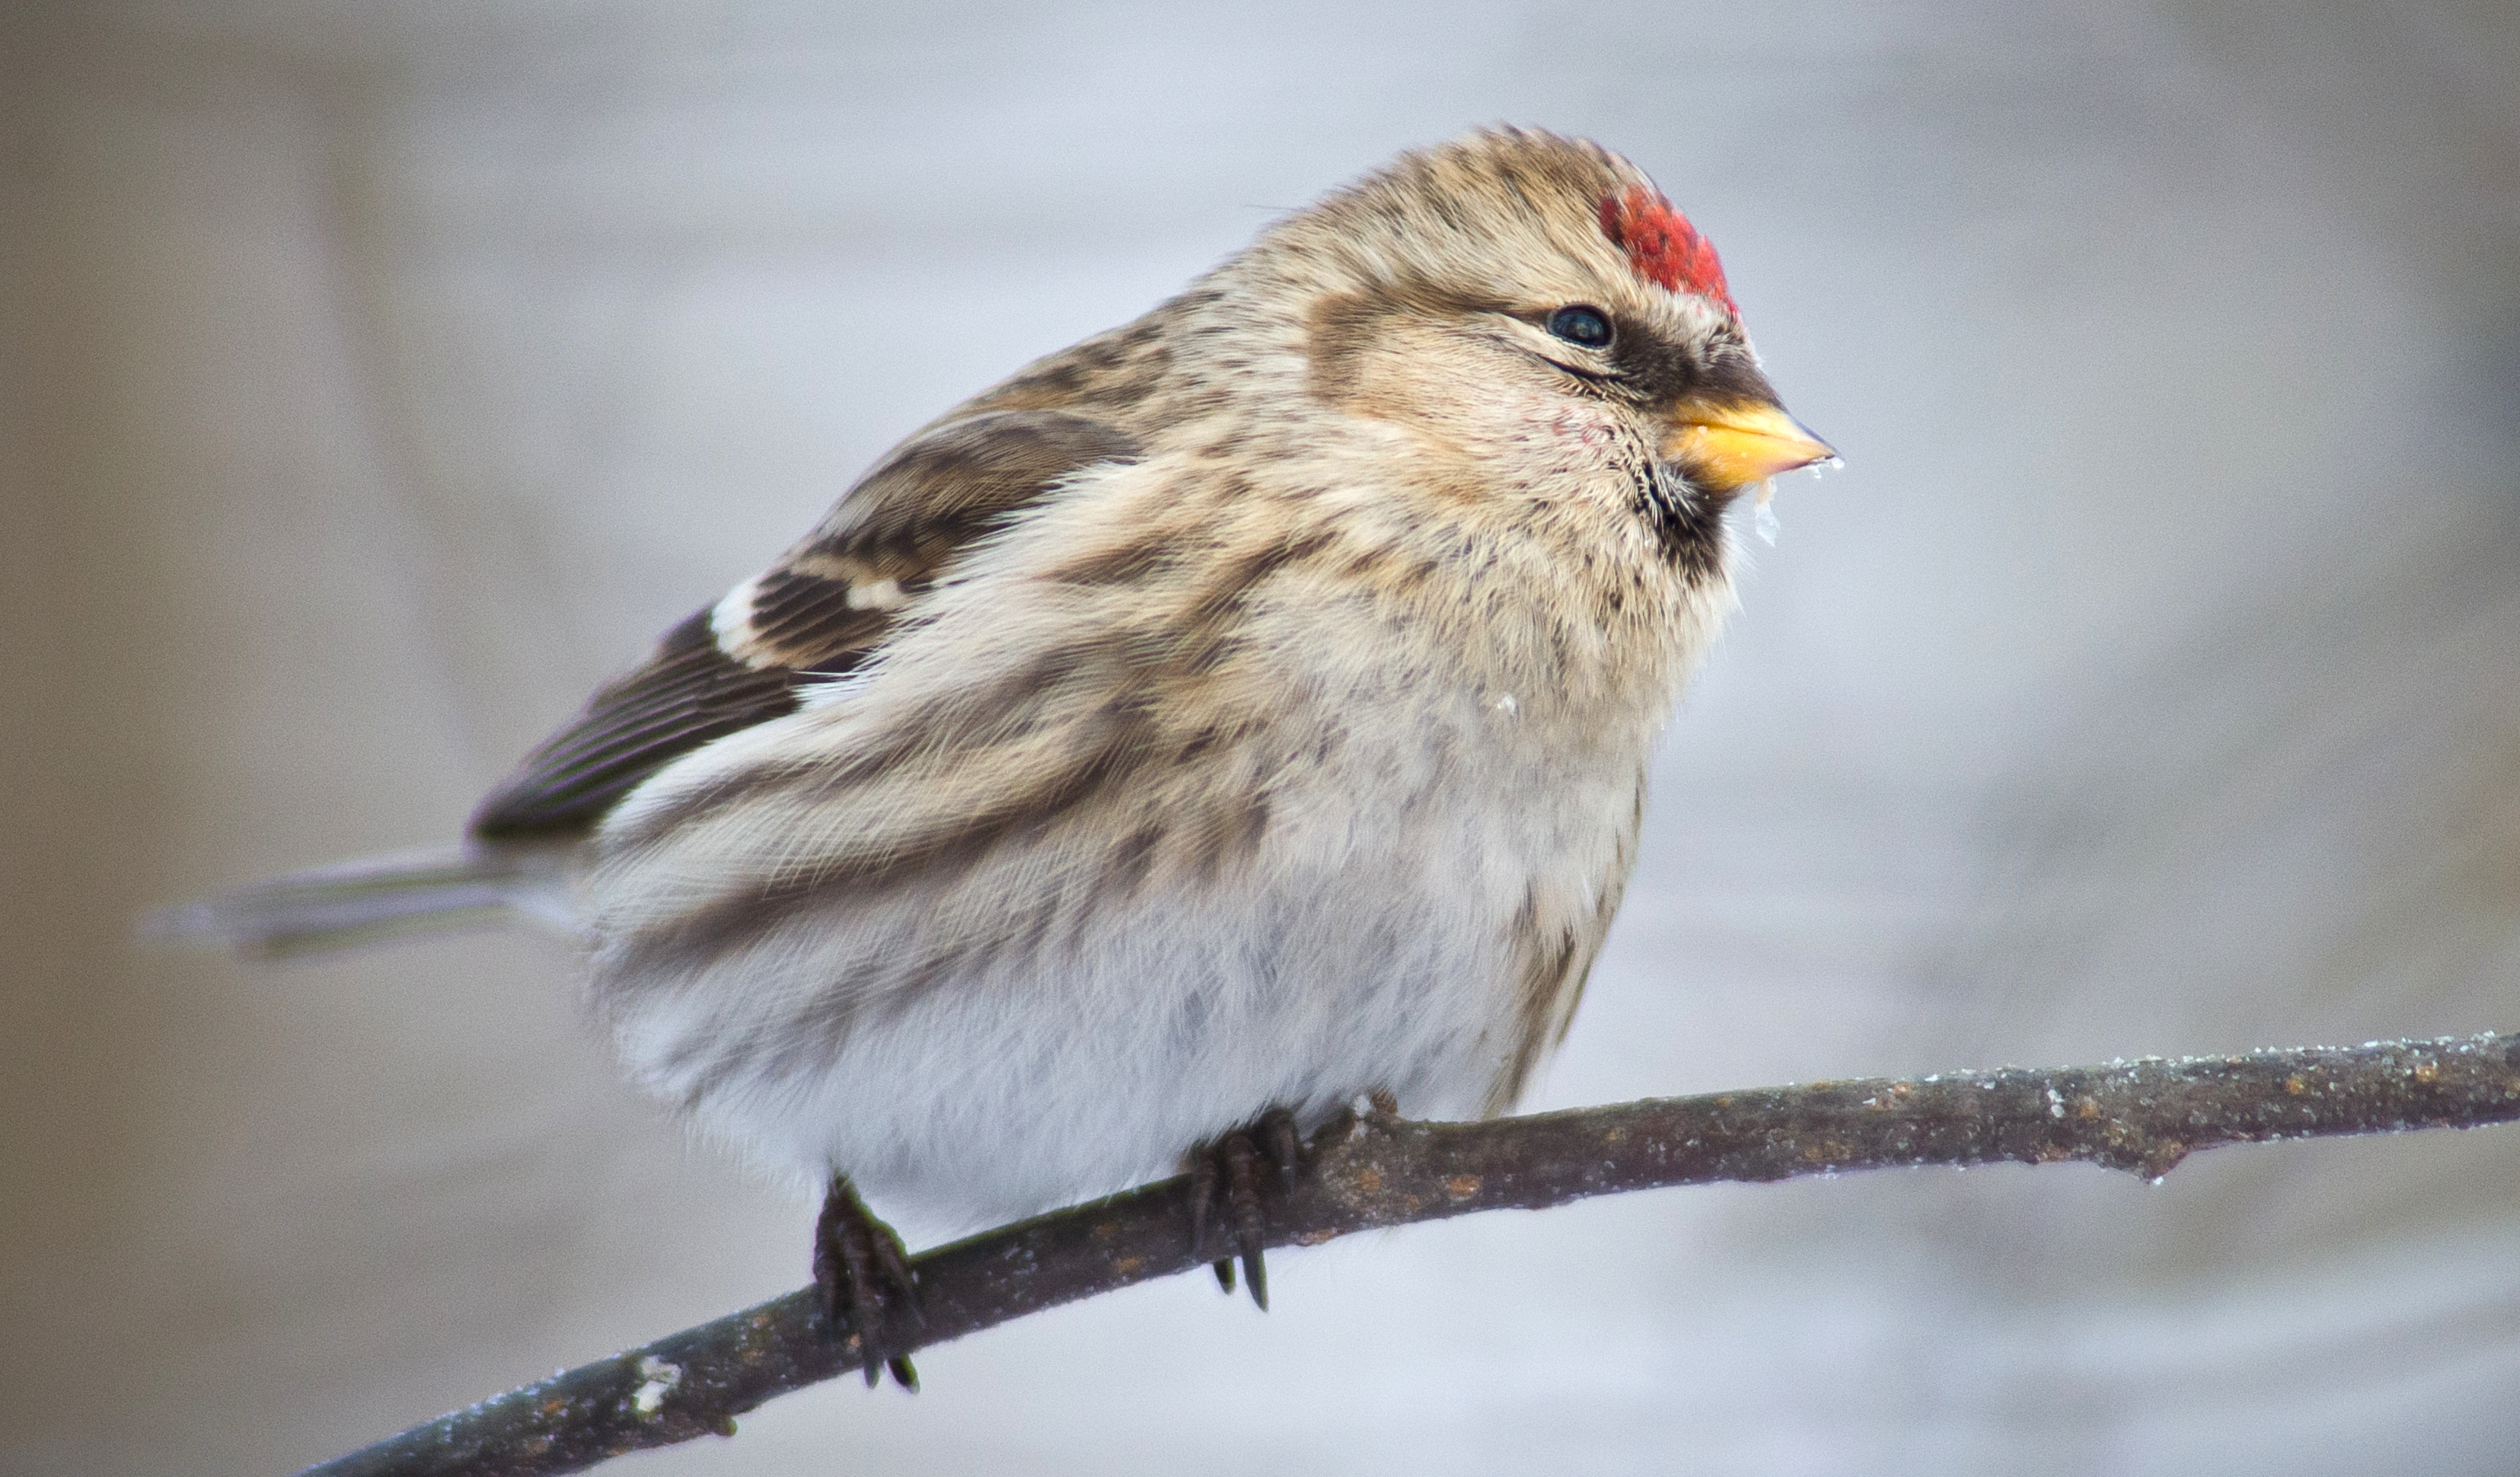
\includegraphics[width=\linewidth]{Acanthis_flammea}
        \caption{A common redpoll (Acanthis Flammea)}
        \label{fig:Acanthis_flammea}
    \end{figure}

\end{center}
\vspace{\baselineskip}

%Students info
\normalsize
\vspace*{\fill}
\begin{flushright}
    Niek R. Scholten (388602)\\
    Bio-Informatics BFV3\\
    Institute of Life Science \& Technology\\
    Hanze University of Applied Sciences\\
    Dave Langers (LADR) \& Bart Barnard (BABA)\\
    \today
\end{flushright}
\newpage

%Blank page
\null
\thispagestyle{empty}
\addtocounter{page}{-1}
\newpage

\begin{center}

%Titles

    \Huge{Predicting bird species from their songs using machine learning}\\
    \vspace{\baselineskip}
    \LARGE{Theme 09 - Introduction Machine Learning}\\
    \vspace{\baselineskip}

\end{center}
\vspace{\baselineskip}

%Students info
\normalsize
\vspace*{\fill}
\begin{flushright}
    Niek R. Scholten (388602)\\
    Bio-Informatics BFV3\\
    Institute of Life Science \& Technology\\
    Hanze University of Applied Sciences\\
    Dave Langers (LADR) \& Bart Barnard (BABA)\\
    \today
\end{flushright}
\newpage

\pagenumbering{roman}
\section*{Abstract}

Here goes the abstract.

\label{sec:abstract}~\addcontentsline{toc}{section}{\nameref{sec:abstract}}
\newpage

\section*{Summary}

Here goes the summary.

\label{sec:summ}~\addcontentsline{toc}{section}{\nameref{sec:summ}}
\newpage

\section*{List of Abbreviations}

\textbf{TEST} Test abbreviation.

\label{sec:abvs}~\addcontentsline{toc}{section}{\nameref{sec:abvs}}

\newpage

{
\setcounter{tocdepth}{2}
\tableofcontents
}
\newpage

\pagenumbering{arabic}

\hypertarget{introduction}{%
\section{Introduction}\label{introduction}}

\hypertarget{purpose}{%
\subsection{Purpose}\label{purpose}}

Here goes the purpose.

\hypertarget{theory}{%
\subsection{Theory}\label{theory}}

Here goes the theory.

\newpage

\hypertarget{materials-methods}{%
\section{Materials \& Methods}\label{materials-methods}}

Here goes the intro for materials \& methods.

\hypertarget{materials}{%
\subsection{Materials}\label{materials}}

Here goes the meterials.

\hypertarget{methods}{%
\subsection{Methods}\label{methods}}

Here goes the methods.

\newpage

\hypertarget{results}{%
\section{Results}\label{results}}

Here goes the results.

\newpage

\hypertarget{conclusion}{%
\section{Conclusion}\label{conclusion}}

Here goes the cunclusion.

\newpage

\hypertarget{discussion}{%
\section{Discussion}\label{discussion}}

Here goes the discussion.

\newpage

\end{document}
